The DGMPM is now illustrated on numerical examples considering materials whose constitutive models are governed by the Hencky hyperelastic potential \cite{Laurent2009}:
\begin{equation}
    \psi = ?
\end{equation}
combined with isotropic hardening. 

The material parameters used are gathered in table \ref{tab:material}.
\begin{table}[h!]
  \centering
    \begin{tabular}{l|l|lN}
    \hline
    $E=2\times 10^{11}\:Pa$ & $\sigma^y=4 \times 10^8 Pa$ & $n=4.37$&  \\ [3pt]
    $\nu=0.3$ & $H=10^{10} Pa$ & $\eta=\sigma^y \:\tau^{1/n} \: Pa.s$ & \\[3pt]
    $\rho = 7800 \: kg.m^{-3}$ & & &\\[3pt]
    \hline
  \end{tabular}

%%% Local Variables:
%%% mode: latex
%%% TeX-master: "../../mainManuscript"
%%% End:

  \caption{Material parameters.}
  \label{tab:material}
\end{table}

\subsection{Plane wave problem}
\label{sec:plane-wave-problem}
Let's first look at the response of a infinite medium in directions $\vect{e}_2$ and $\vect{e}_3$, and length $l=1\:m$ in direction $\vect{e}_1$ to Riemann-type initial conditions on the velocity: $v_1=v_d>0$ for $x\in[0,L/2[$ and $v_1=-v_d$ for $x \in ]L/2,L]$.
The solid is initially in a free stress state and the initial velocity is set so that plastic flow occurs:
\begin{equation*}
  v_d=1.2\frac{Y_H}{\rho c_L}
\end{equation*}
where $Y_H=(\lambda+2\mu)\sigma^y/2\mu$ denotes the Hugoniot elastic limit, $c_L=\sqrt{(\lambda+2\mu)/\rho}$ is the elastic pressure wave speed, and $(\lambda,\mu)$ are Lam\'e's constants. Both ends of the medium are traction free.
%so that rightward and leftward compressive elastic waves reflect as unloading waves that interact with the incident plastic ones \cite{Thomas_EVP}.

The initial setting is assumed to give rise to a plane wave, namely:
\begin{align*}
  & \tens{F}= F \vect{e}_1 \otimes\vect{e}_1 + \vect{e}_2 \otimes\vect{e}_2 + \vect{e}_3 \otimes\vect{e}_3\\
  & \tens{\Pi}=\Pi_L \vect{e}_1 \otimes \vect{e}_1 + \Pi_T \(\vect{e}_2 \otimes \vect{e}_2+\vect{e}_3 \otimes \vect{e}_3\) 
\end{align*}
%In that configuration, a relation exists between longitudinal and transverse stress components $\Pi_L$ and $\Pi_T$ in such a way that a one-dimensional hyperbolic system is solved for $\Pi_L=\Pi$, and the transverse component $\Pi_T$ is computed subsequently. 
In the linearized geometrical limit $\norm{\tens{F}} \ll 1$, the computed hyperelastic-plastic solution should tend to the elastoplastic one derived in \cite{Thomas_EP}.
The latter consists of two elastic compression waves propagating left and right-ward, each followed by one plastic discontinuity.
The incident elastic disturbances then reflect as unloading waves on both free boundaries of the domain, the interaction of which at the center of the medium leads to tensile plastic reloading.


\begin{figure}[ht]
  \centering
  \begin{tikzpicture}[spy using outlines={rectangle, magnification=3, size=1.cm, connect spies},scale=.8]
  \begin{groupplot}[group style={group size=3 by 2,ylabels at=edge left, yticklabels at=edge left,horizontal sep=2.ex,vertical sep=4ex,xticklabels at=edge bottom,xlabels at=edge bottom},ymajorgrids=true,xmajorgrids=true,enlargelimits=0,xmin=0.5,xmax=1.,xlabel=$x (m)$,axis on top,scale only axis,width=0.33\linewidth,height=0.25\linewidth]

    % ============================== Stress Line
    % t1 % t= 6.84e-5
    \nextgroupplot[title={(a) $t = 6.84\times 10^{-5} $ s.},ylabel=$\Pi_L \: (Pa)$,ymin=-8.5e8,ymax=8.e8]
    \addplot[Red,densely dashed,thick] table[x=x,y=Pi] {pgfFigures/HEP_planeWave/mpm0.pgf};
    \addplot[Green,densely dotted,very thick] table[x=x,y=Pi] {pgfFigures/HEP_planeWave/mpm_2ppc0.pgf};
    \addplot[Blue,mark=asterisk,thick,mark repeat=2,mark size=3pt] table[x=x,y=Pi] {pgfFigures/HEP_planeWave/dgmpm0.pgf};
    %\addplot[Purple,mark=x,thick,mark repeat=2,mark size=3pt] table[x=x,y=Pi] {pgfFigures/HEP_planeWave/dgmpm_2ppc0.pgf};
    \addplot[Purple,mark=x,thick,mark repeat=2,mark size=3pt] table[x=x,y=Pi] {pgfFigures/HEP_planeWave/dgmpm_2ppc_effective0.pgf};
    \addplot[Orange,mark=*,thick,mark repeat=2,mark size=2pt] table[x=x,y=Pi] {pgfFigures/HEP_planeWave/fem0.pgf};
    \addplot[black] table[x=x,y=Pi] {pgfFigures/HEP_planeWave/exact0.pgf};

    \begin{scope}
      \spy[black,size=1.5cm] on (2.8,0.25) in node [fill=none] at (2.725,3.);
    \end{scope}

    % t2 % t= 1.37e-4
    \nextgroupplot[title={(b) $t=1.37\times 10^{-4}$ s.},ymin=-8.5e8,ymax=8.e8]
    \addplot[Red,densely dashed,thick] table[x=x,y=Pi] {pgfFigures/HEP_planeWave/mpm1.pgf};
    \addplot[Green,densely dotted,very thick] table[x=x,y=Pi] {pgfFigures/HEP_planeWave/mpm_2ppc1.pgf};
    \addplot[Blue,mark=asterisk,thick,mark repeat=2,mark size=3pt] table[x=x,y=Pi] {pgfFigures/HEP_planeWave/dgmpm1.pgf};
    \addplot[Purple,mark=x,thick,mark repeat=2,mark size=3pt] table[x=x,y=Pi] {pgfFigures/HEP_planeWave/dgmpm_2ppc1.pgf};
    %\addplot[Yellow,mark=+,thick,mark repeat=2,mark size=3pt] table[x=x,y=Pi] {pgfFigures/HEP_planeWave/dgmpm_2ppc_effective1.pgf};
    \addplot[Orange,mark=*,thick,mark repeat=2,mark size=2pt] table[x=x,y=Pi] {pgfFigures/HEP_planeWave/fem1.pgf};
    \addplot[black] table[x=x,y=Pi] {pgfFigures/HEP_planeWave/exact1.pgf};


    % \begin{scope}
    %   \spy[black,size=1.5cm] on (7.2,1.5) in node [fill=none] at (6.75,3.);
    % \end{scope}

    
    % t3 % t= 2.05e-4
    \nextgroupplot[title={(c) $t=2.05\times 10^{-4}$ s.},ymin=-8.5e8,ymax=8.e8]
    \addplot[Red,densely dashed,thick] table[x=x,y=Pi] {pgfFigures/HEP_planeWave/mpm2.pgf};
    \addplot[Green,densely dotted,very thick] table[x=x,y=Pi] {pgfFigures/HEP_planeWave/mpm_2ppc2.pgf};
    \addplot[Blue,mark=asterisk,thick,mark repeat=2,mark size=3pt] table[x=x,y=Pi] {pgfFigures/HEP_planeWave/dgmpm2.pgf};
    \addplot[Purple,mark=x,thick,mark repeat=2,mark size=3pt] table[x=x,y=Pi] {pgfFigures/HEP_planeWave/dgmpm_2ppc2.pgf};
    %\addplot[Yellow,mark=+,thick,mark repeat=2,mark size=3pt] table[x=x,y=Pi] {pgfFigures/HEP_planeWave/dgmpm_2ppc_effective2.pgf};
    \addplot[Orange,mark=*,thick,mark repeat=2,mark size=2pt] table[x=x,y=Pi] {pgfFigures/HEP_planeWave/fem2.pgf};
    \addplot[black] table[x=x,y=Pi] {pgfFigures/HEP_planeWave/exact2.pgf};
    
    % \begin{scope}
    %   \spy[black,size=1.5cm] on (9.65+2.,3.5) in node [fill=none] at (11+3.2,1.25);
    % \end{scope}

    % ============================== Plastic strain Line
    % t1
    \nextgroupplot[ylabel=$E^p_{11}$,ymin=-1.12e-3,ymax=2.e-4]
    \addplot[Red,densely dashed,thick] table[x=x,y=epls] {pgfFigures/HEP_planeWave/mpm0.pgf};
    \addplot[Green,densely dotted,very thick] table[x=x,y=epls] {pgfFigures/HEP_planeWave/mpm_2ppc0.pgf};
    \addplot[Blue,mark=asterisk,thick,mark repeat=2,mark size=3pt] table[x=x,y=epls] {pgfFigures/HEP_planeWave/dgmpm0.pgf};
    \addplot[Purple,mark=x,thick,mark repeat=2,mark size=3pt] table[x=x,y=epls] {pgfFigures/HEP_planeWave/dgmpm_2ppc0.pgf};
    %\addplot[Yellow,mark=+,thick,mark repeat=2,mark size=3pt] table[x=x,y=epls] {pgfFigures/HEP_planeWave/dgmpm_2ppc_effective0.pgf};
    \addplot[Orange,mark=*,thick,mark repeat=2,mark size=2pt] table[x=x,y=epls] {pgfFigures/HEP_planeWave/fem0.pgf};
    \addplot[black] table[x=x,y=epls] {pgfFigures/HEP_planeWave/exact0.pgf};
    
    % t2
    \nextgroupplot[legend style={at={($(0.9,-0.45)+(2.1cm,0.65cm)$)},legend columns=3},ymin=-1.12e-3,ymax=2.e-4]
    \addplot[Red,densely dashed,thick] table[x=x,y=epls] {pgfFigures/HEP_planeWave/mpm1.pgf};
    \addplot[Green,densely dotted,very thick] table[x=x,y=epls] {pgfFigures/HEP_planeWave/mpm_2ppc1.pgf};
    \addplot[Blue,mark=asterisk,thick,mark repeat=2,mark size=3pt] table[x=x,y=epls] {pgfFigures/HEP_planeWave/dgmpm1.pgf};
    \addplot[Purple,mark=x,thick,mark repeat=2,mark size=3pt] table[x=x,y=epls] {pgfFigures/HEP_planeWave/dgmpm_2ppc1.pgf};
    %\addplot[Yellow,mark=+,thick,mark repeat=2,mark size=3pt] table[x=x,y=epls] {pgfFigures/HEP_planeWave/dgmpm_2ppc_effective1.pgf};
    
    \addplot[Orange,mark=*,thick,mark repeat=2,mark size=2pt] table[x=x,y=epls] {pgfFigures/HEP_planeWave/fem1.pgf};
    \addplot[black] table[x=x,y=epls] {pgfFigures/HEP_planeWave/exact1.pgf};
    
    \addlegendentry{mpm (1ppc)}
    \addlegendentry{mpm (2ppc)}
    \addlegendentry{dgmpm (1ppc)}
    \addlegendentry{dgmpm (2ppc)}
    %\addlegendentry{dgmpm (2ppc) -- effective}
    \addlegendentry{fem}
    \addlegendentry{exact}
    % t3
    \nextgroupplot[,ymin=-1.12e-3,ymax=2.e-4]
    \addplot[Red,densely dashed,thick] table[x=x,y=epls] {pgfFigures/HEP_planeWave/mpm2.pgf};
    \addplot[Green,densely dotted,very thick] table[x=x,y=epls] {pgfFigures/HEP_planeWave/mpm_2ppc2.pgf};
    \addplot[Blue,mark=asterisk,thick,mark repeat=2,mark size=3pt] table[x=x,y=epls] {pgfFigures/HEP_planeWave/dgmpm2.pgf};
    \addplot[Purple,mark=x,thick,mark repeat=2,mark size=3pt] table[x=x,y=epls] {pgfFigures/HEP_planeWave/dgmpm_2ppc2.pgf};
    %\addplot[Yellow,mark=+,thick,mark repeat=2,mark size=3pt] table[x=x,y=epls] {pgfFigures/HEP_planeWave/dgmpm_2ppc_effective2.pgf};
    
    \addplot[Orange,mark=*,thick,mark repeat=2,mark size=2pt] table[x=x,y=epls] {pgfFigures/HEP_planeWave/fem2.pgf};
    \addplot[black] table[x=x,y=epls] {pgfFigures/HEP_planeWave/exact2.pgf};

  \end{groupplot}
\end{tikzpicture}



%%% Local Variables:
%%% mode: latex
%%% TeX-master: "../manuscript"
%%% End:

  \label{fig:hep_planeWave}
  \caption{Longitudinal components of PK1 stress and plastic Green-Lagrange strain tensors along a one-dimensional hyperelastic-plastic domain subject to Riemann-type initial conditions on the velocity at different times. Comparison between FEM (CFL=1), MPM (CFL=0.7), DGMPM using one particle per cell (CFL=1) of four particles per cell (CFL=0.5), and the exact solution of the small strain problem.}
\end{figure}

\begin{figure}[ht]
  \centering
  \begin{tikzpicture}[scale=.8]
  \begin{groupplot}[group style={group size=3 by 2,ylabels at=edge left, yticklabels at=edge left,horizontal sep=2.ex,vertical sep=4ex,xticklabels at=edge bottom,xlabels at=edge bottom},ymajorgrids=true,xmajorgrids=true,enlargelimits=0,xmin=0.,xmax=1.,xlabel=$x (m)$,axis on top,scale only axis,width=0.33\linewidth]

    % ============================== Stress Line
    % t1 % t= 6.84e-5
    \nextgroupplot[title={(a) $t = 6.75\times 10^{-5} $ s.},ylabel=$\Pi_L \: (Pa)$,ymin=-3.e9,ymax=0.]
    \addplot[Red,densely dashed,thick] table[x=x,y=Pi] {pgfFigures/HEP_planeWave/mpm_high_0.pgf};
    \addplot[Blue,mark=asterisk,thick,mark repeat=2,mark size=2pt] table[x=x,y=Pi] {pgfFigures/HEP_planeWave/dgmpm_high_0.pgf};
    \addplot[Purple,mark=x,thick,mark repeat=2,mark size=2pt] table[x=x,y=Pi] {pgfFigures/HEP_planeWave/dgmpm_2ppc_high_0.pgf};
    \addplot[Orange,mark=*,thick,mark repeat=2,mark size=1pt] table[x=x,y=Pi] {pgfFigures/HEP_planeWave/fem_high_0.pgf};
    %\addplot[black] table[x=x,y=Pi] {pgfFigures/HEP_planeWave/exact_high_0.pgf};
    
    % t2 % t= 1.37e-4
    \nextgroupplot[title={(b) $t=1.35\times 10^{-4}$ s.},ymin=-3e9,ymax=0.]
    \addplot[Red,densely dashed,thick] table[x=x,y=Pi] {pgfFigures/HEP_planeWave/mpm_high_1.pgf};
    \addplot[Blue,mark=asterisk,thick,mark repeat=2,mark size=2pt] table[x=x,y=Pi] {pgfFigures/HEP_planeWave/dgmpm_high_1.pgf};
    \addplot[Purple,mark=x,thick,mark repeat=2,mark size=2pt] table[x=x,y=Pi] {pgfFigures/HEP_planeWave/dgmpm_2ppc_high_1.pgf};
    \addplot[Orange,mark=*,thick,mark repeat=2,mark size=1pt] table[x=x,y=Pi] {pgfFigures/HEP_planeWave/fem_high_1.pgf};
    %\addplot[black] table[x=x,y=Pi] {pgfFigures/HEP_planeWave/exact_high_1.pgf};

    % t3 % t= 2.05e-4
    \nextgroupplot[title={(c) $t=2.05\times 10^{-4}$ s.},ymin=-3e9,ymax=0.]
    \addplot[Red,densely dashed,thick] table[x=x,y=Pi] {pgfFigures/HEP_planeWave/mpm_high_2.pgf};
    \addplot[Blue,mark=asterisk,thick,mark repeat=2,mark size=2pt] table[x=x,y=Pi] {pgfFigures/HEP_planeWave/dgmpm_high_2.pgf};
    \addplot[Purple,mark=x,thick,mark repeat=2,mark size=2pt] table[x=x,y=Pi] {pgfFigures/HEP_planeWave/dgmpm_2ppc_high_2.pgf};
    \addplot[Orange,mark=*,thick,mark repeat=2,mark size=1pt] table[x=x,y=Pi] {pgfFigures/HEP_planeWave/fem_high_2.pgf};
    %\addplot[black] table[x=x,y=Pi] {pgfFigures/HEP_planeWave/exact_high_2.pgf};

    % ============================== Plastic strain Line
    % t1
    \nextgroupplot[ylabel=$E^p_{11}$,ymin=-0.9e-2,ymax=0.]
    \addplot[Red,densely dashed,thick] table[x=x,y=epls] {pgfFigures/HEP_planeWave/mpm_high_0.pgf};
    \addplot[Blue,mark=asterisk,thick,mark repeat=2,mark size=2pt] table[x=x,y=epls] {pgfFigures/HEP_planeWave/dgmpm_high_0.pgf};
    \addplot[Purple,mark=x,thick,mark repeat=2,mark size=2pt] table[x=x,y=epls] {pgfFigures/HEP_planeWave/dgmpm_2ppc_high_0.pgf};
    \addplot[Orange,mark=*,thick,mark repeat=2,mark size=1pt] table[x=x,y=epls] {pgfFigures/HEP_planeWave/fem_high_0.pgf};
    %\addplot[black] table[x=x,y=epls] {pgfFigures/HEP_planeWave/exact_high_0.pgf};
    
    % t2
    \nextgroupplot[legend style={at={($(0.9,-0.45)+(2.25cm,1cm)$)},legend columns=5},ymin=-0.9e-2,ymax=0.]
    \addplot[Red,densely dashed,thick] table[x=x,y=epls] {pgfFigures/HEP_planeWave/mpm_high_1.pgf};
    \addplot[Blue,mark=asterisk,thick,mark repeat=2,mark size=2pt] table[x=x,y=epls] {pgfFigures/HEP_planeWave/dgmpm_high_1.pgf};
    \addplot[Purple,mark=x,thick,mark repeat=2,mark size=2pt] table[x=x,y=epls] {pgfFigures/HEP_planeWave/dgmpm_2ppc_high_1.pgf};
    
    \addplot[Orange,mark=*,thick,mark repeat=2,mark size=1pt] table[x=x,y=epls] {pgfFigures/HEP_planeWave/fem_high_1.pgf};
    %\addplot[black] table[x=x,y=epls] {pgfFigures/HEP_planeWave/exact_high_1.pgf};
    
    \addlegendentry{mpm}
    \addlegendentry{dgmpm (1ppc)}
    \addlegendentry{dgmpm (2ppc)}
    \addlegendentry{fem}
    %\addlegendentry{exact}
    % t3
    \nextgroupplot[,ymin=-0.9e-2,ymax=0.] % 3.e-3 if exact solution is depicted
    \addplot[Red,densely dashed,thick] table[x=x,y=epls] {pgfFigures/HEP_planeWave/mpm_high_2.pgf};
    \addplot[Blue,mark=asterisk,thick,mark repeat=2,mark size=2pt] table[x=x,y=epls] {pgfFigures/HEP_planeWave/dgmpm_high_2.pgf};
    \addplot[Purple,mark=x,thick,mark repeat=2,mark size=2pt] table[x=x,y=epls] {pgfFigures/HEP_planeWave/dgmpm_2ppc_high_2.pgf};
    
    \addplot[Orange,mark=*,thick,mark repeat=2,mark size=1pt] table[x=x,y=epls] {pgfFigures/HEP_planeWave/fem_high_2.pgf};
    %\addplot[black] table[x=x,y=epls] {pgfFigures/HEP_planeWave/exact_high_2.pgf};

  \end{groupplot}
\end{tikzpicture}



%%% Local Variables:
%%% mode: latex
%%% TeX-master: "../manuscript"
%%% End:

  \label{fig:hep_planeWave_high}
  \caption{Check times of computation}
\end{figure}
Constant speed for the exact solution while it's not the case.

\subsection{Plane strain problem}
\label{sec:plane-strain-problem}
%% Comparison at t=0.00102126

\begin{figure}[ht]
  \centering
  \subcaptionbox{Geometry and boundary conditions\label{subfig:2D_domain}}{\begin{tikzpicture}[scale=1.]
  \draw[thick] (0,0) --(3,0)--(3,3)--(0,3)--(0,0);
  \foreach \x in {0.5,1.,...,2.5} 
  \draw(\x,-0.2)circle(0.2);
  \foreach \x in {0.25,0.75,...,2.75} 
  \draw(-0.2,\x)circle(0.2);
  \draw(0,-0.4)--(3.,-0.4);
  \draw(-.4,0)--(-.4,3);
  \fill [pattern=north east lines](0.0,-0.8)rectangle+(3,0.4);
  \fill [pattern=north east lines](-.8,0.)rectangle+(0.4,3);
  \draw[>=stealth,<->](0,3.1)--node[above=1pt]{\footnotesize $l=3 \: m$}(3,3.1);
  %\draw[>=stealth,<->](0.1,0)--node[right=1pt]{\footnotesize $a=1 \: m$}(0.1,1);
  % \foreach \x in {0.,0.25,...,1} 
  % \draw[>=stealth,<-] (-0.5,\x)--(0.,\x);
  % \node(a)at(-1.75,0.5){\footnotesize $\vect{v}=\matrice{v^d\\0 \\0}$}; 
  \node[right] (a) at(3.25,1.5){\footnotesize $\vect{v}(\vect{X},t=0)=\matrice{v_d\\0 \\0}$}; 
  \draw[>=stealth,->](-2.5,2)--(-1.5,2)node(a)[anchor=north]{\footnotesize $\vect{e}_1$};
  \draw[>=stealth,->](-2.5,2)--(-2.5,3)node(a)[anchor=south]{\footnotesize $\vect{e}_2$};
\end{tikzpicture}


%%% Local Variables:
%%% mode: latex
%%% TeX-master: "../manuscript"
%%% End:
}
  \subcaptionbox{Material points set and grids \label{subfig:2d_meshes}}{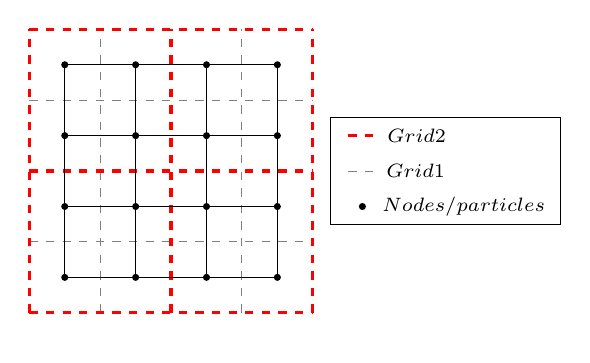
\begin{tikzpicture}[scale=0.9]
  \draw (0,0) --(3,0)--(3,3)--(0,3)--(0,0);
  \draw[white] (0.,0) -- (0,-0.8);
  %%% Grid 1
  \foreach \y in {-0.5,0.5,...,3.5} 
  \draw[dashed,gray] (-0.5,\y) -- (3.5,\y);
  \foreach \x in {-0.5,0.5,...,3.5} 
  \draw[dashed,gray] (\x,-0.5) -- (\x,3.5);
  %%% Grid 2
  \foreach \y in {-0.5,1.5,...,3.5} 
  \draw[dashed,Red,very thick] (-0.5,\y) -- (3.5,\y);
  \foreach \x in {-0.5,1.5,...,3.5} 
  \draw[dashed,Red,very thick] (\x,-0.5) -- (\x,3.5);
  \foreach \y in {0.,1.,...,3.} 
  \foreach \x in {0.,1.,...,3.} 
  \fill (\x,\y) circle(0.05);
  \foreach \y in {0.,1.,...,3.} 
  \draw (0,\y) -- (3.,\y);
  \foreach \x in {0.,1.,...,3.} 
  \draw (\x,0) -- (\x,3);
  \draw (3.75,0.75) rectangle (7.,2.25);
  \fill (4.2,1.) circle (0.05) node [right] {\scriptsize$ \: \: \text{Nodes / particles}$};
  \draw[dashed,gray] (4.,1.5) -- (4.4,1.5) node [right] {\scriptsize$\color{black} \text{Grid 1}$};
  \draw[dashed,very thick,Red] (4.,2.) -- (4.4,2.) node [right] {\scriptsize$\color{black} \text{Grid 2}$};
\end{tikzpicture}


%%% Local Variables:
%%% mode: latex
%%% TeX-master: "../manuscript"
%%% End:
}
  \caption{domain}
  \label{fig:PS_domain}
\end{figure}


Il faut faire une breve analyse de convergence ?

\begin{figure}[ht]
  \centering
  \subcaptionbox{Stress}{\begin{tikzpicture}[scale=1]
  \begin{groupplot}[group style={group size=2 by 4,% columns by rows
      ylabels at=edge left, yticklabels at=edge left,
      horizontal sep=5.ex,
      vertical sep=2ex,},
    enlargelimits=0,
    xmin=0.,xmax=1., ymin=-0.,ymax=1.
    ,axis on top,scale only axis,width=0.18\linewidth
    ,xtick=\empty,ytick=\empty,
    colorbar style={
      title style={
        font=\normalsize,
        at={(1,.5)},
        anchor=north west
      },yticklabel style={font=\normalsize}
      ,at={(current axis.south east)},anchor=south west
    },colormap name=tol
    ]
    %% FIRST ROW (time 1 = 5.10e-4s)
    %%% RANGE -8.6e9 -- 0.57e9
    \nextgroupplot[title={$t=5.10\times 10^{-4} \:s$},ylabel={FEM}]\addplot graphics[xmin=0.,xmax=1., ymin=-0.,ymax=1.] {pngFigures/fem_stress1-crop.png};
    \nextgroupplot[title={$t=1.02\times 10^{-3} \:s$}]\addplot graphics[xmin=0.,xmax=1., ymin=-0.,ymax=1.] {pngFigures/fem_stress2-crop.png};

    \nextgroupplot[ylabel={MPM(1ppc)}]\addplot graphics[xmin=0.,xmax=1., ymin=-0.,ymax=1.] {pngFigures/mpm1ppc_stress1-crop.png};
    \nextgroupplot[]\addplot graphics[xmin=0.,xmax=1., ymin=-0.,ymax=1.] {pngFigures/mpm1ppc_stress2-crop.png};

    \nextgroupplot[ylabel={DGMPM(1ppc)}]\addplot graphics[xmin=0.,xmax=1., ymin=-0.,ymax=1.] {pngFigures/dgmpm1ppc_stress1-crop.png};
    \nextgroupplot[]\addplot graphics[xmin=0.,xmax=1., ymin=-0.,ymax=1.] {pngFigures/dgmpm1ppc_stress2-crop.png};
    

    \nextgroupplot[ylabel={DGMPM(4ppc)},colorbar horizontal,colorbar  style={
      title style={yshift=-1.5cm},
      title= {$\Pi_{11}\: (GPa)$},
      xtick={-8.6,0.56},
      xticklabels={-8.6,0.56},
    }]
    \addplot[scatter,scatter src=x,mark size=0.pt] coordinates {(-8.6,0.) (0.56,0)};% Fake extreme values to fix scale
    \addplot graphics[xmin=0.,xmax=1., ymin=-0.,ymax=1.] {pngFigures/dgmpm4ppc_stress1-crop.png};
    \nextgroupplot[colorbar horizontal,colorbar  style={
      title style={yshift=-1.5cm},
      title= {$\Pi_{11}\: (GPa)$},
      xtick={-3,7.6},
      xticklabels={-3,7.6},
    }]
    \addplot[scatter,scatter src=x,mark size=0.pt] coordinates {(-3.,0.) (7.6,0)};% Fake extreme values to fix scale
    \addplot graphics[xmin=0.,xmax=1., ymin=-0.,ymax=1.] {pngFigures/dgmpm4ppc_stress2-crop.png};
    
  \end{groupplot}
\end{tikzpicture}



%%% Local Variables:
%%% mode: latex
%%% TeX-master: "../manuscript"
%%% End:
}
  \subcaptionbox{Cumulated plastic strain}{\begin{tikzpicture}[scale=1]
  \begin{groupplot}[group style={group size=2 by 4,% columns by rows
      ylabels at=edge left, yticklabels at=edge left,
      horizontal sep=5.ex,
      vertical sep=2ex,},
    enlargelimits=0,
    xmin=0.,xmax=1., ymin=-0.,ymax=1.
    ,axis on top,scale only axis,xtick=\empty,ytick=\empty,width=0.18\linewidth,
    colorbar style={
      title style={
        font=\normalsize,
        at={(1,.5)},
        anchor=north west
      },yticklabel style={font=\normalsize}
      ,at={(current axis.south east)},anchor=south west
    },colormap name=tol]
    %% FIRST ROW (time 1 = 5.10e-4s)
    %%% RANGE -8.6e9 -- 0.57e9
    \nextgroupplot[title={$t=5.10\times 10^{-4} \:s$},ylabel={FEM}]\addplot graphics[xmin=0.,xmax=1., ymin=-0.,ymax=1.] {pngFigures/fem_epeq1-crop.png};
    \nextgroupplot[title={$t=1.02\times 10^{-3} \:s$}]\addplot graphics[xmin=0.,xmax=1., ymin=-0.,ymax=1.] {pngFigures/fem_epeq2-crop.png};

    \nextgroupplot[ylabel={MPM}]\addplot graphics[xmin=0.,xmax=1., ymin=-0.,ymax=1.] {pngFigures/mpm_epeq1-crop.png};
    \nextgroupplot[]\addplot graphics[xmin=0.,xmax=1., ymin=-0.,ymax=1.] {pngFigures/mpm_epeq2-crop.png};

    \nextgroupplot[ylabel={DGMPM--1ppc}]\addplot graphics[xmin=0.,xmax=1., ymin=-0.,ymax=1.] {pngFigures/dgmpm1ppc_epeq1-crop.png};
    \nextgroupplot[]\addplot graphics[xmin=0.,xmax=1., ymin=-0.,ymax=1.] {pngFigures/dgmpm1ppc_epeq2-crop.png};
    

    \nextgroupplot[ylabel={DGMPM--4ppc},colorbar horizontal,colorbar  style={
      title style={yshift=-1.5cm},
      title= {$p$},
      xtick={0,.15},
      xticklabels={0,0.15},
    }]
    \addplot[scatter,scatter src=x,mark size=0.pt] coordinates {(0,0.) (0.15,0)};% Fake extreme values to fix scale
    \addplot graphics[xmin=0.,xmax=1., ymin=-0.,ymax=1.] {pngFigures/dgmpm4ppc_epeq1-crop.png};
    \nextgroupplot[colorbar horizontal,colorbar  style={
      title style={yshift=-1.5cm},
      title= {$p$},
      xtick={0.,0.16},
      xticklabels={0,0.16},
    }]
    \addplot[scatter,scatter src=x,mark size=0.pt] coordinates {(0.,0.) (0.16,0)};% Fake extreme values to fix scale
    \addplot graphics[xmin=0.,xmax=1., ymin=-0.,ymax=1.] {pngFigures/dgmpm4ppc_epeq2-crop.png};
    
  \end{groupplot}
\end{tikzpicture}



%%% Local Variables:
%%% mode: latex
%%% TeX-master: "../manuscript"
%%% End:
}
  \caption{Isovalues of the PK1 stress tensor component $\Pi_{11}$ and cumulated plastic strain in a two-dimensional hyperelastic-plastic solids impacting a rigid wall under plane strain. Comparison of FEM (CFL=0.9), MPM (CFL=0.7) and DGMPM solutions using either one particle per cell (CFL=1) or four particles per cell (CFL=0.4).}
  \label{fig:test}
\end{figure}


\begin{figure}[ht]
  \centering
  \begin{tikzpicture}
  \begin{groupplot}[group style={group size=2 by 2, % 3 columns 2 rows
      ylabels at=edge left, yticklabels at=edge left,horizontal sep=2.ex,vertical sep=5.ex,
      xticklabels at=edge bottom,xlabels at=edge bottom},
    ymajorgrids=true,xmajorgrids=true,
    axis on top,scale only axis,width=0.425\linewidth,
    height=0.25\linewidth,
    every x tick scale label/.style={at={(xticklabel* cs:1.05,0.75cm)},anchor=near yticklabel},
    every y tick scale label/.style={at={(yticklabel* cs:1.05,-.9cm)},anchor=near yticklabel}]
    
    %%%%%%%%%%%%%%%%%%%% 
    % ============================== Stress Line
    % t1 
    \nextgroupplot[ylabel=$\Pi_{11} \:(Pa)$,title={(a) $t = 5.10 \times 10^{-4}\: s$},ymin=-1.e10,ymax=7.25e9]
    \addplot[Orange,thick,mark=*,mark repeat=2] table[x=Points:0,y=Piola_Stress:0] {csvFiles/fem_bottom1.csv};
    \addplot[Red,thick,mark=square,only marks] table[x=Points:0,y=Piola:0] {csvFiles/mpm_bottom1.csv};
    \addplot[black!60,thick,mark=o,only marks] table[x=Points:0,y=Piola:0] {csvFiles/mpm4ppc_bottom1.csv};
    \addplot[Blue,thick,mark=asterisk,only marks,mark size=3pt] table[x=Points:0,y=PK1:0] {csvFiles/dgmpm1ppc_bottom1.csv};
    \addplot[Purple,thick,mark=x,only marks,mark size=3pt,mark repeat=2] table[x=Points:0,y=PK1:0] {csvFiles/dgmpm4ppc_bottom1.csv};
    
    % t2 
    \nextgroupplot[title={(b) $t = 1.02 \times 10^{-3}\: s$},ymin=-1.e10,ymax=7.25e9%,ymin=-7.5e9,ymax=100.e9,ytick scale label code/.code={},legend style={at={($(0.75,-0.4)+(0.9cm,0.6cm)$)},legend columns=3}
    ]
    \addplot[Orange,thick,mark=*,mark repeat=2] table[x=Points:0,y=Piola_Stress:0] {csvFiles/fem_bottom2.csv};
    \addplot[Red,thick,mark=square,only marks] table[x=Points:0,y=Piola:0] {csvFiles/mpm_bottom2.csv};
    \addplot[black!60,thick,mark=o,only marks] table[x=Points:0,y=Piola:0] {csvFiles/mpm4ppc_bottom2.csv};
    \addplot[Blue,thick,mark=asterisk,only marks,mark size=3pt] table[x=Points:0,y=PK1:0] {csvFiles/dgmpm1ppc_bottom2.csv};
    \addplot[Purple,thick,mark=x,only marks,mark size=3pt,mark repeat=2] table[x=Points:0,y=PK1:0] {csvFiles/dgmpm4ppc_bottom2.csv};


    % ============================== Cumulated plastic strain Line
    % t1 
    \nextgroupplot[ylabel=$p$,xlabel=$x_1 \: (m)$,ymin=0.,ymax=9.e-2%,ymin=-7.5e9,ymax=100.e9,ytick scale label code/.code={}
    ]
    \addplot[Orange,thick,mark=*,mark repeat=2] table[x=Points:0,y=Equivalent_Plastic_Strain] {csvFiles/fem_bottom1.csv};
    \addplot[Red,thick,mark=square,only marks] table[x=Points:0,y=epeq] {csvFiles/mpm_bottom1.csv};
    \addplot[black!60,thick,mark=o,only marks] table[x=Points:0,y=epeq] {csvFiles/mpm4ppc_bottom1.csv};
    \addplot[Blue,thick,mark=asterisk,only marks,mark size=3pt] table[x=Points:0,y=epeq] {csvFiles/dgmpm1ppc_bottom1.csv};
    \addplot[Purple,thick,mark=x,only marks,mark size=3pt,mark repeat=2] table[x=Points:0,y=epeq] {csvFiles/dgmpm4ppc_bottom1.csv};
    
    % t2
    \nextgroupplot[legend style={at={($(0.75,-0.35)+(0.2cm,0.35cm)$)},legend columns=5},xlabel=$x_1 \: (m)$,ymin=0.,ymax=9.e-2%,ymin=-7.5e9,ymax=100.e9,ytick scale label code/.code={}
    ]
    \addplot[Orange,thick,mark=*,mark repeat=2] table[x=Points:0,y=Equivalent_Plastic_Strain] {csvFiles/fem_bottom2.csv};
    \addplot[Red,thick,mark=square,only marks] table[x=Points:0,y=epeq] {csvFiles/mpm_bottom2.csv};
    \addplot[black!60,thick,mark=o,only marks] table[x=Points:0,y=epeq] {csvFiles/mpm4ppc_bottom2.csv};
    \addplot[Blue,thick,mark=asterisk,only marks,mark size=3pt] table[x=Points:0,y=epeq] {csvFiles/dgmpm1ppc_bottom2.csv};
    \addplot[Purple,thick,mark=x,only marks,mark size=3pt,mark repeat=2] table[x=Points:0,y=epeq] {csvFiles/dgmpm4ppc_bottom2.csv};

    \addlegendentry{fem \:}
    \addlegendentry{mpm (1ppc) \:}
    \addlegendentry{mpm (4ppc) \:}
    \addlegendentry{dgmpm (1ppc) \:}
    \addlegendentry{dgmpm (4ppc) \:}
    
    
  \end{groupplot}
\end{tikzpicture}



%%% Local Variables:
%%% mode: latex
%%% TeX-master: "../manuscript"
%%% End:

  \caption{Comparison of the longitudinal stress component and cumulated plastic strain along the bottom boundary of the domain at two different times}
  \label{fig:bottom_line}
\end{figure}

\begin{figure}[ht]
  \centering
  \begin{tikzpicture}
  \begin{groupplot}[group style={group size=2 by 2, % 3 columns 2 rows
      ylabels at=edge left, yticklabels at=edge left,horizontal sep=2.ex,vertical sep=3.ex,
      xticklabels at=edge bottom,xlabels at=edge bottom},
    ymajorgrids=true,xmajorgrids=true,
    axis on top,scale only axis,width=0.425\linewidth, every x tick scale label/.style={at={(xticklabel* cs:1.05,0.75cm)},anchor=near yticklabel},
    every y tick scale label/.style={at={(yticklabel* cs:1.05,-0.9cm)},anchor=near yticklabel}]
    
    %%%%%%%%%%%%%%%%%%%% 
    % ============================== Stress Line
    % t1 
    \nextgroupplot[ylabel=$\Pi_{11} \:(Pa)$,title={(a) $t = 5.10 \times 10^{-4}\: s$},ymin=-8.5e9,ymax=2.e9]
    \addplot[Orange,thick,mark=*,mark repeat=2] table[x=Points:1,y=Piola_Stress:0] {csvFiles/fem_left1.csv};
    \addplot[Red,thick,mark=square,only marks] table[x=Points:1,y=Piola:0] {csvFiles/mpm_left1.csv};
    \addplot[black!60,thick,mark=o,only marks] table[x=Points:1,y=Piola:0] {csvFiles/mpm4ppc_left1.csv};
    \addplot[Blue,thick,mark=asterisk,only marks,mark size=3pt] table[x=Points:1,y=PK1:0] {csvFiles/dgmpm1ppc_left1.csv};
    \addplot[Purple,thick,mark=x,only marks,mark size=3pt,mark repeat=2] table[x=Points:1,y=PK1:0] {csvFiles/dgmpm4ppc_left1.csv};
    
    % t2 
    \nextgroupplot[title={(b) $t = 1.02 \times 10^{-3}\: s$},ymin=-8.5e9,ymax=2.e9%,ymin=-7.5e9,ymax=100.e9,ytick scale label code/.code={},legend style={at={($(0.75,-0.4)+(0.9cm,0.6cm)$)},legend columns=3}
    ]
    \addplot[Orange,thick,mark=*,mark repeat=2] table[x=Points:1,y=Piola_Stress:0] {csvFiles/fem_left2.csv};
    \addplot[Red,thick,mark=square,only marks] table[x=Points:1,y=Piola:0] {csvFiles/mpm_left2.csv};
    \addplot[black!60,thick,mark=o,only marks] table[x=Points:1,y=Piola:0] {csvFiles/mpm4ppc_left2.csv};
    \addplot[Blue,thick,mark=asterisk,only marks,mark size=3pt] table[x=Points:1,y=PK1:0] {csvFiles/dgmpm1ppc_left2.csv};
    \addplot[Purple,thick,mark=x,only marks,mark size=3pt,mark repeat=2] table[x=Points:1,y=PK1:0] {csvFiles/dgmpm4ppc_left2.csv};


    % ============================== Cumulated plastic strain Line
    % t1 
    \nextgroupplot[ylabel=$p$,xlabel=$y \: (m)$,ymin=2.e-2,ymax=1.8e-1%,ymin=-7.5e9,ymax=100.e9,ytick scale label code/.code={}
    ]
    \addplot[Orange,thick,mark=*,mark repeat=2] table[x=Points:1,y=Equivalent_Plastic_Strain] {csvFiles/fem_left1.csv};
    \addplot[Red,thick,mark=square,only marks] table[x=Points:1,y=epeq] {csvFiles/mpm_left1.csv};
    \addplot[black!60,thick,mark=o,only marks] table[x=Points:1,y=epeq] {csvFiles/mpm4ppc_left1.csv};
    \addplot[Blue,thick,mark=asterisk,only marks,mark size=3pt] table[x=Points:1,y=epeq] {csvFiles/dgmpm1ppc_left1.csv};
    \addplot[Purple,thick,mark=x,only marks,mark size=3pt,mark repeat=2] table[x=Points:1,y=epeq] {csvFiles/dgmpm4ppc_left1.csv};
    
    % t2
    \nextgroupplot[legend style={at={($(0.75,-0.35)+(0.cm,1cm)$)},legend columns=5},xlabel=$y \: (m)$,ymin=2.e-2,ymax=1.8e-1%,ymin=-7.5e9,ymax=100.e9,ytick scale label code/.code={}
    ]
    \addplot[Orange,thick,mark=*,mark repeat=2] table[x=Points:1,y=Equivalent_Plastic_Strain] {csvFiles/fem_left2.csv};
    \addplot[black!60,thick,mark=o,only marks] table[x=Points:1,y=epeq] {csvFiles/mpm_left2.csv};
    \addplot[Red,thick,mark=square,only marks] table[x=Points:1,y=epeq] {csvFiles/mpm4ppc_left2.csv};
    \addplot[Blue,thick,mark=asterisk,only marks,mark size=3pt] table[x=Points:1,y=epeq] {csvFiles/dgmpm1ppc_left2.csv};
    \addplot[Purple,thick,mark=x,only marks,mark size=3pt,mark repeat=2] table[x=Points:1,y=epeq] {csvFiles/dgmpm4ppc_left2.csv};

    \addlegendentry{fem \:}
    \addlegendentry{mpm (1ppc) \:}
    \addlegendentry{mpm (4ppc) \:}
    \addlegendentry{dgmpm (1ppc) \:}
    \addlegendentry{dgmpm (4ppc) \:}
    
    
  \end{groupplot}
\end{tikzpicture}



%%% Local Variables:
%%% mode: latex
%%% TeX-master: "../manuscript"
%%% End:

  \caption{Comparison of the longitudinal stress component and cumulated plastic strain along the left boundary of the domain at two different times}
  \label{fig:left_line}
\end{figure}

\subsection{Non-linear hardening material}
\label{sec:non-linear-hardening}
Reprendre le cas test hyperelastique de la these?


%%% Local Variables:
%%% mode: latex
%%% TeX-master: "manuscript"
%%% End:
